%\documentclass{article}
\documentclass{easychair}
\newtheorem{hypothesis}{Hypothesis}
\usepackage{graphicx}
\usepackage{url}
\usepackage[show]{ed}

\usepackage{helvet}
\usepackage{xcolor}
\usepackage{graphbox}
\usepackage{tikz}

% RGB
\newcommand{\mkc}[4]{\definecolor{#1}{RGB}{#4}}

%%%%%%%%%%%%%%%%%%%%%%%%%%%%%%%%%%%%%%%%%%%%%%%%%%%%%%%%%%%%%%%%%%%%%%%%%%%%%%
% Colours, text macros and similar stuff
%%%%%%%%%%%%%%%%%%%%%%%%%%%%%%%%%%%%%%%%%%%%%%%%%%%%%%%%%%%%%%%%%%%%%%%%%%%%%%

%%%%%%%%%%%%%%%%%%%%%%%%%%%%%%%%%%%%%%%%%%%%%%%%%%%%%%%%%%%%%%%%%%%%%%%%%%%%%%
% Non-Altran Colours
%%%%%%%%%%%%%%%%%%%%%%%%%%%%%%%%%%%%%%%%%%%%%%%%%%%%%%%%%%%%%%%%%%%%%%%%%%%%%%

% A very light grey for pxcode
\definecolor{CodeBG}{rgb}{0.95,0.95,0.95}

%%%%%%%%%%%%%%%%%%%%%%%%%%%%%%%%%%%%%%%%%%%%%%%%%%%%%%%%%%%%%%%%%%%%%%%%%%%%%%
% New 2017 Style
%%%%%%%%%%%%%%%%%%%%%%%%%%%%%%%%%%%%%%%%%%%%%%%%%%%%%%%%%%%%%%%%%%%%%%%%%%%%%%

\mkc{Altran1} {PANTONE 2185C}{  1, .38, .17, .02}{0,118,165}   % altran blue
\mkc{Altran2} {PANTONE 2915C}{.60, .09,   0,   0}{98,181,229}  % light blue
\mkc{Altran3} {PANTONE 393C} {.06,   0, .55,   0}{240,236,116} % pale yellow
\mkc{Altran4} {PANTONE 381C} {.25,   0, .98,   0}{206,220,0}   % yellow/green
\mkc{Altran5} {PANTONE 7506C}{  0  .07, .25, .01}{239,219,178} % beige
\mkc{Altran6} {PANTONE 7670C}{.80, .74,   0,   0}{86,82,148}   % purple
\mkc{Altran7} {PANTONE 116C} {  0  .14,   1,   0}{255,205,0}   % yellow
\mkc{Altran8} {PANTONE 631C} {.74,   0, .13,   0}{62,177,200}  % mid blue
\mkc{Altran9} {PANTONE 5415C}{.56, .24, .11, .34}{91,127,149}  % grey blue
\mkc{Altran10}{PANTONE 1787C}{  0, .82, .53,   0}{244,54,76}   % bright red
\mkc{Altran11}{PANTONE 5275C}{.74, .68, .07, .31}{89,84,120}   % dark purple
\mkc{Altran12}{PANTONE 214C} {  0,   1, .24, .04}{206,15,105}  % offensive red

\colorlet{AnColour01}{Altran1}
\colorlet{AnColour02}{Altran2}
\colorlet{AltranTitle}{Altran6}

%%%%%%%%%%%%%%%%%%%%%%%%%%%%%%%%%%%%%%%%%%%%%%%%%%%%%%%%%%%%%%%%%%%%%%%%%%%%%%
% Compatibility: Altran UK Style (up to 2016)
%%%%%%%%%%%%%%%%%%%%%%%%%%%%%%%%%%%%%%%%%%%%%%%%%%%%%%%%%%%%%%%%%%%%%%%%%%%%%%

\colorlet{AltranSubtitle}{Altran11}
\colorlet{AltranGrey}{Altran9}

\colorlet{AnGrey01}{Altran11!20}
\colorlet{AnGrey02}{Altran11!40}
\colorlet{AnGrey03}{Altran11!20}
\colorlet{AnGrey04}{Altran11!80}
\colorlet{AnGrey05}{Altran11}

\colorlet{AnSecondaryRed}   {Altran10}
\colorlet{AnSecondaryGreen} {Altran4}
\colorlet{AnSecondaryPurple}{Altran6}
\colorlet{AnSecondaryYellow}{Altran7}

\colorlet{AnSecondary01}{AnSecondaryRed}
\colorlet{AnSecondary02}{AnSecondaryGreen}
\colorlet{AnSecondary03}{AnSecondaryPurple}
\colorlet{AnSecondary04}{AnSecondaryYellow}

%%%%%%%%%%%%%%%%%%%%%%%%%%%%%%%%%%%%%%%%%%%%%%%%%%%%%%%%%%%%%%%%%%%%%%%%%%%%%%
% Compatibility: Praxis
%%%%%%%%%%%%%%%%%%%%%%%%%%%%%%%%%%%%%%%%%%%%%%%%%%%%%%%%%%%%%%%%%%%%%%%%%%%%%%

\colorlet{PraxisPurple}{Altran6}
\colorlet{PraxisPink}{Altran12}


%\usepackage{tikz}
\usepackage{amsfonts}
\usetikzlibrary{datavisualization}
\pgfdvdeclarestylesheet{altran}{
  1/.style={Altran1},
  2/.style={Altran4},
  3/.style={Altran6},
  4/.style={Altran7},
  5/.style={Altran8},
  6/.style={Altran12},
  default style/.style={black}
}
\bibliographystyle{plain}
\begin{document}
\title{Benchmarking Solvers, SAT-style}
\author{Martin Nyx Brain\inst{1} \and James H. Davenport\inst{2} \and Alberto Griggio\inst{3}}
\institute{ 
University of Oxford, Oxford, U.K. {\tt Martin.Brain@cs.ox.ac.uk} \and
University of Bath, Bath, U.K. {\tt J.H.Davenport@bath.ac.uk} \and
Fondazione Bruno Kessler, Trento, Italy {\tt griggio@fbk.eu}}
\authorrunning{Brain/Davenport/Griggio}
\titlerunning{Benchmarking}
\maketitle
\begin{abstract}\noindent
The SAT community, and hence the SMT community, have substantial experience in benchmarking solvers against each other on large sample sets, and publishing summaries, whereas the computer algebra community tends to time solvers on a small set of problems, and publishing individual times.
\par
This paper aims to document the SAT community practice for the benefit of the computer algebra community.
\end{abstract}
\input BenchInner
\section{Virtual Best Solver}
Though not shown in  Figure  \ref{fig:survivor}, the SAT competition has taken to including a "virtual best solver" (VBS)
which is synthesised from the other results by taking the minimum (across all solvers tested) time taken to solve every given benchmark.
Thus the VBS time is always equal to the time of some real solver, but which one will change by the benchmark (measuring how often each solver is the VBS is also an interesting metric).  The VBS can be added to the survivor/cactus plot to get a feeling for the variability between solvers. In particular, if it tracks one solver, then that is close to being the best, whereas if it does significantly better than any individual solver, that is an indication that the different real solvers have different strengths and weaknesses, and a portfolio approach might be appropriate. See Section \ref{sec:RL}.
\par
We have therefore added this to our solvers on the diagrams, and counted how often a solver is the VBS. A variation on counting is provided by \cite{Janotaetal2016a}, who measure how often a solver is within one second of being VBS. Their justification is ``The constant of one second was chosen since we consider a smaller difference as insignificant, especially in the context of 800 second time-out''.
%\ednote{@All: do we want to discuss this? For example, this is just as subject to random fluctuation as the original, but in a different place. How about scoring ``VBS points'': 1 if VBS, 0 if more than 5\% slower than VBS, and linear in between? Or any other smooth idea?}
This is open to the argument that it is just as subject to random fluctuation as the original, but in a different place. One could consider scoring ``VBS points'': 1 if VBS, 0 if more than 5\% slower\footnote{A percentage-based approach is probably more appropriate than a fixed time, as differences in time tend to come from consistent features. But this could also do with more experimentation.} than VBS, and linear  interpolation in between.
\section{Running multiple copies}
One of the effects of having a solution process whose running time is widely variable\footnote{These algorithms are widely called \emph{Las Vegas} algorithms. However, the term has different connotations in the different fields. In Symbolic Computation, most Las Vegas algorithms are ones that normally produce the answer in a deterministically-bounded time, but may occcasionally fail and have to try again, and effort goes into bounding the error probability, and proving that the algorithm will terminate. Modular algorithms are a classic example. But here we are considering algorithms whose running time is intrinsically variable.} is that one may well not be best served by just running the process to termination.  In the case of a single processor, this issue was considered by \cite{Lubyetal1993}, who suggested (and indeed proved almost-optimality) running the process up to certain time limits and then starting afresh, where the limits were  of the form $T,T,2T,T,T,2T,4T,T,T,2T,T,T,2T,4T,8T,\ldots$, where $T$ is some arbitrary unit.
\par
This is in fact the default behaviour in MiniSAT 2.2.0, where it is known as \verb+Luby+ (though $T$ is in fact measured in terms of conflicts rather than time, and it's not a complete restart that is performed, as certain learned clauses are kept). 
\par
These days, with processors getting more numerous rather than faster, we might consider running multiple copies in parallel. To see how this might help, consider the trivial case of a process whose running time is $1,K,K^2$ with equal probability. Then the average time to solution is $\frac13(1+K+K^2)=37$ when $K=10$. Running two copies and aborting the other when one finds the solution has an average time to solution of $\frac19(5+3K+K^2)=15$ when $K=10$, so the CPU cost is 30 units, still less than the sequential cost.
Similarly, three copies gives $\frac1{27}(19+7K+K^2)=7$ when $K=10$, so the CPU cost is 21 units, even better.  For $K=10$, the minimum is achieved at 8-fold parallelism, with time-to-solution 1.36 units, and a CPU cost of 10.9 units.

The break even point for two-fold parallel running is $K=\frac12\left(1+\sqrt{37}\right)\approx4.5$, and three-fold running is $K=4$. It is worth noting, though, that a single Luby process with $T=\frac13$ (to avoid $T=1$ getting lucky) achieves an average time to solution (and cost) of $\approx 9$.
\section{Distributions}
\subsection{Normal Distribution of Times}\label{sec:Normal}
\begin{figure}[h]
\caption{Data from Section \ref{sec:Normal} --- Normal distribution\label{Fig:Normal}}
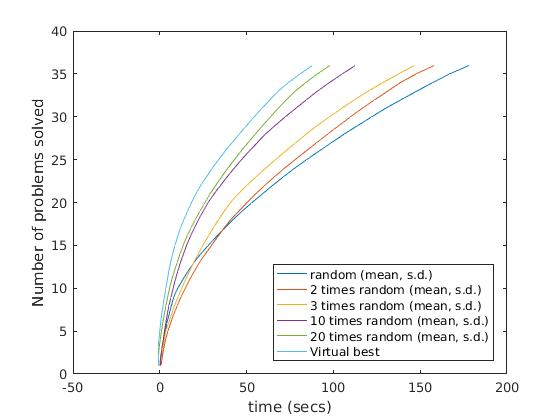
\includegraphics[scale=0.4]{RSolve20.jpg}
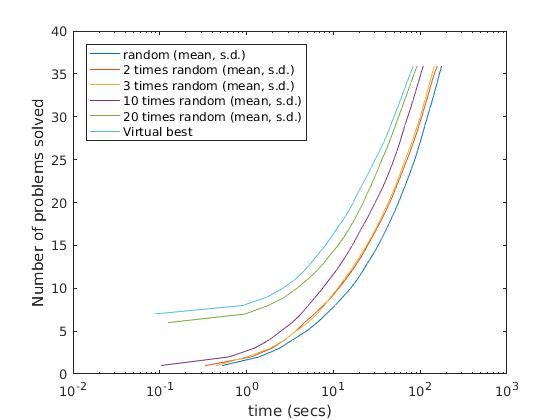
\includegraphics[scale=0.4]{RlogSolve20.jpg}
\end{figure}
It is far from clear what sort of distribution the running times of SAT, and even less SMT, solvers have, but it would be foolish to ignore the normal distribution. We took 36 hypothetical cases, with 9 different running times $t_0=1,\ldots,9$, and standard deviations $t_0/10,2t_0/10,3t_0/10,4t_0/10$ for each running time. The mean running times roughly mimic the fact that a benchmark suite will have problems of a range of difficulties (indeed, we may have underplayed the range). Some problems seem to be more variable than others,but we have no real justification for the scale of standard deviations.

We used five (hypothetical) possible solvers. The base line one just took a time $t$ at random from the relevant normal distribution: $t \in N(t_0,kt_0/10)$. The second one ran two copies in parallel, terminating when the first one did, the third ran three copies, and the next two 10 and 20. In this case, the VBS is in fact the equivalent of running 36 copies.
The data are in Figure  \ref{Fig:Normal}. Note that we are \emph{not} charging twice for the cost of running two copies, i.e. we are looking at ``time to solution'' not ``cost of solution''
\begin{figure}[h]
\caption{Data from Section \ref{sec:Normal} --- log Normal distribution\label{Fig:Normallog}}
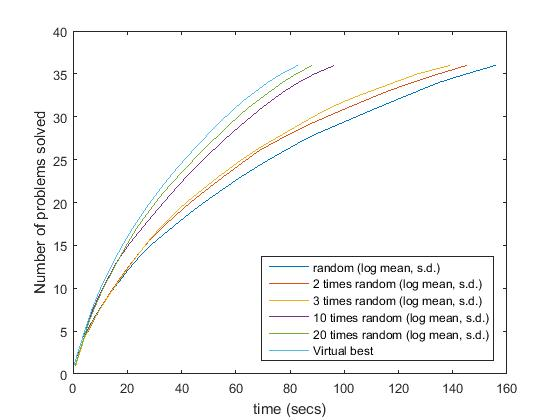
\includegraphics[scale=0.4]{RSolvelog20v2.jpg}
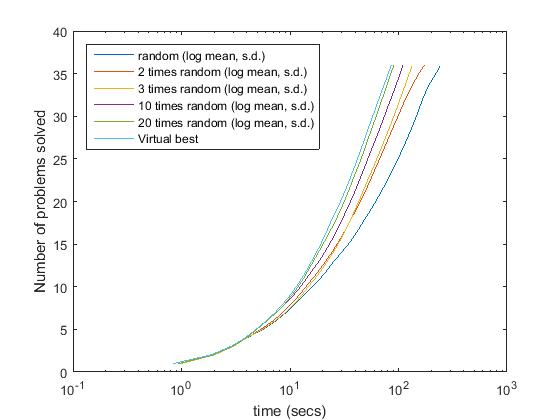
\includegraphics[scale=0.4]{RlogSolvelog20v2.jpg}
\end{figure}

It is also not clear whether we should assume $t$ or $\log t$ is normally distributed. Hence we re-ran these experiments, but applied the normal distribution in $\log t$-space. The standard deviation was scaled so that it bore the same ratio to the mean as before, i.e. $\sigma_{\log}=\sigma\frac{\mu_{\log}}\mu$, where $\mu$ and $\sigma$ represent the mean and standard deviation.
Again, the VBS is in fact the equivalent of running 36 copies.
The data are in Figure  \ref{Fig:Normallog}. We note that the left-hand figures look almost identical, but the right-hand (semi-log plot) ones show a distinct difference at the lower end.
\subsection{Uniform Distribution of Times}\label{sec:Uniform}
\begin{figure}[h]
\caption{Data from Section \ref{sec:Uniform} --- Uniform distribution\label{Fig:Uniform}}
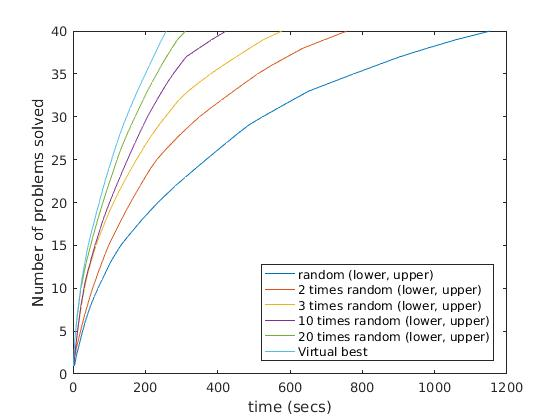
\includegraphics[scale=0.4]{Runif20.jpg}
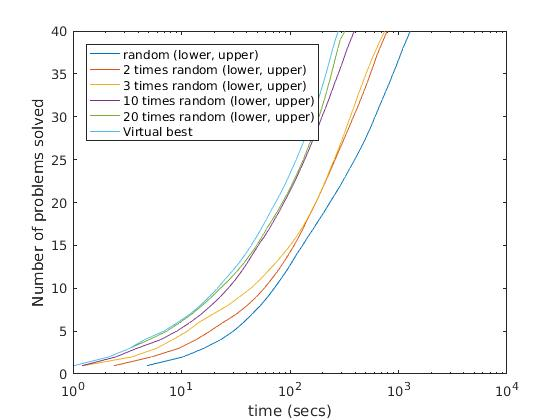
\includegraphics[scale=0.4]{Rlogunif20.jpg}
\end{figure}
We then considered uniform distributions, with the lower bounds being $t_0=1,\ldots,10$, and the upper bounds being 10 times that. We used the same hypothetical solvers as before.
The data are in Figure  \ref{Fig:Uniform}.

Again, one could say that we should be uniform in $\log(t)$, and we did these computations.
The data are in Figure  \ref{Fig:Uniformlog}.
\begin{figure}[h]
\caption{Data from Section \ref{sec:Uniform} --- log Uniform distribution\label{Fig:Uniformlog}}
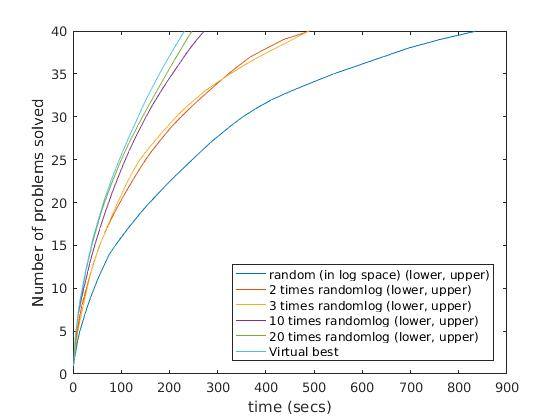
\includegraphics[scale=0.4]{Runiflog20.jpg}
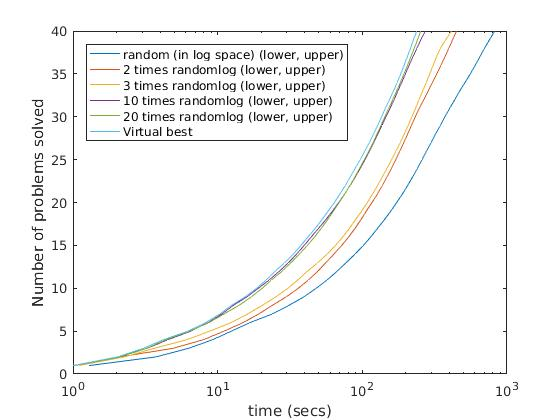
\includegraphics[scale=0.4]{Rloguniflog20.jpg}
\end{figure}
It might seem from these that running twice and running thrice were very similar, and in fact that running twice was almost half the time of running once, thus meaning that they were almost equivalent in cost. In fact, this model is susceptible to algebraic treatment,
and the formulae (running from 1 to $B$ seconds, with numeric values for $B=10$) are as follows:
\begin{equation*}
\begin{array}{rcccl}
\hbox{once}&=&\frac{B-1}{\log B}&\approx&3.9087\\
\hbox{twice}&=&\frac{2}{(\log B)^2}(B-(\log B +1))&\approx&2.5264\\
\hbox{thrice}&=&\frac{6}{(\log B)^3}\left(B-(\frac12\log B+\log B +1)\right)&\approx&1.9887\\
\end{array}
\end{equation*}
Hence in fact the ``running thrice'' number is approximately correct, at one-half the elapsed time of running once.
%\subsection{New}
%Ideas to compare normal and uniform times distributions. Both when $t$ is distributed that way, and when $\log(t)$ is. Also we should look at issues of racing multiple copies, in both cases.
%Normal distrbutions, $t=1,ldots,9$ with standard deviations $t/10,2t/10,3t/10,4t/10$, applied directly or to log.

%Uniform distributions, lower bounds $1,\ldots,10$, upper bounds 10 times that
%\afterpage{
\begin{figure}[h]
\caption{Data from Section \ref{sec:Pr}\label{Fig:S2}}
\hbox{\hskip-60pt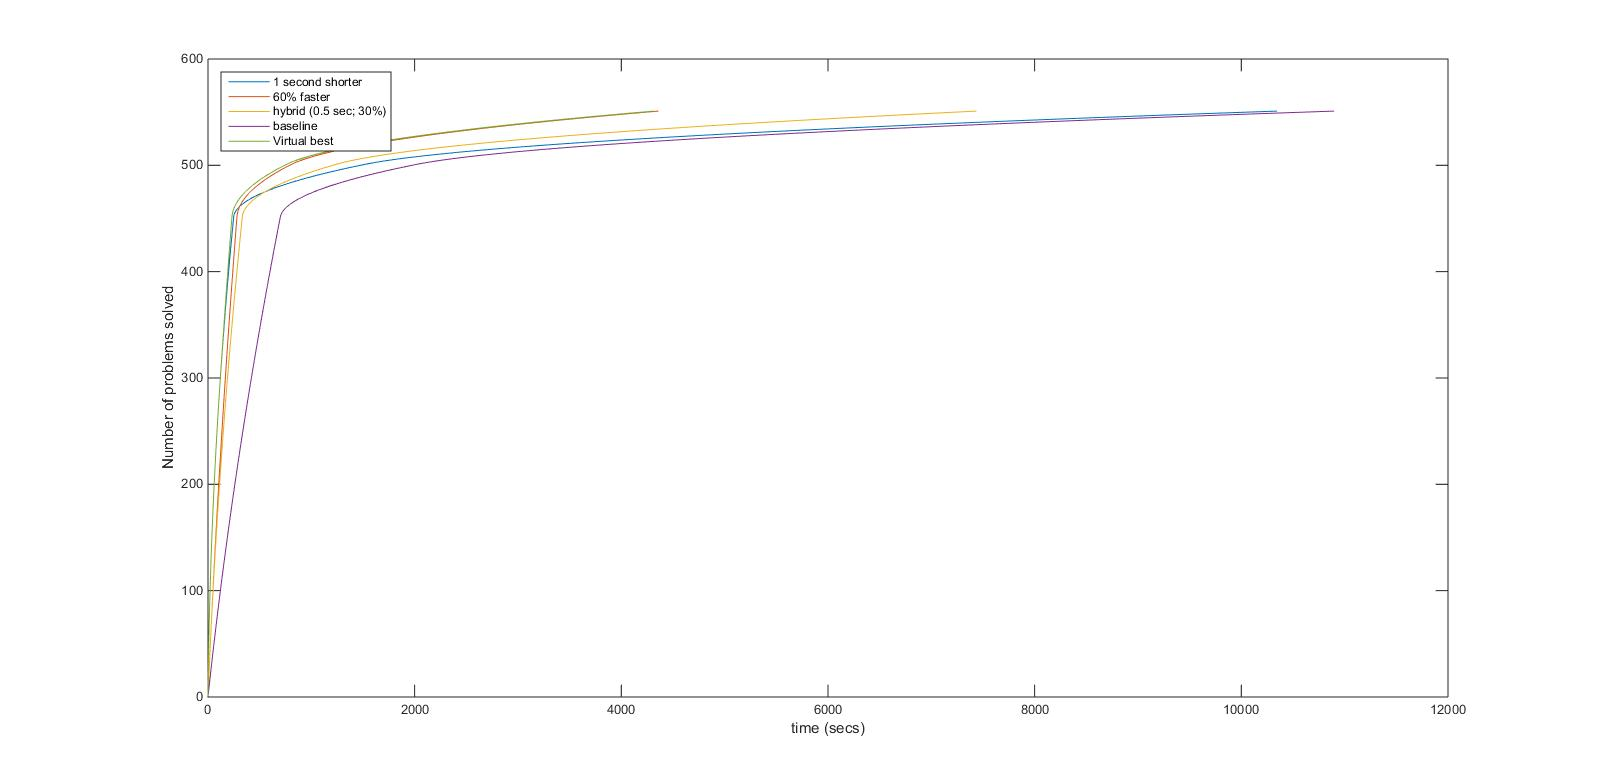
\includegraphics[scale=0.35]{Fig2a.jpg}}
\hbox{\hskip-60pt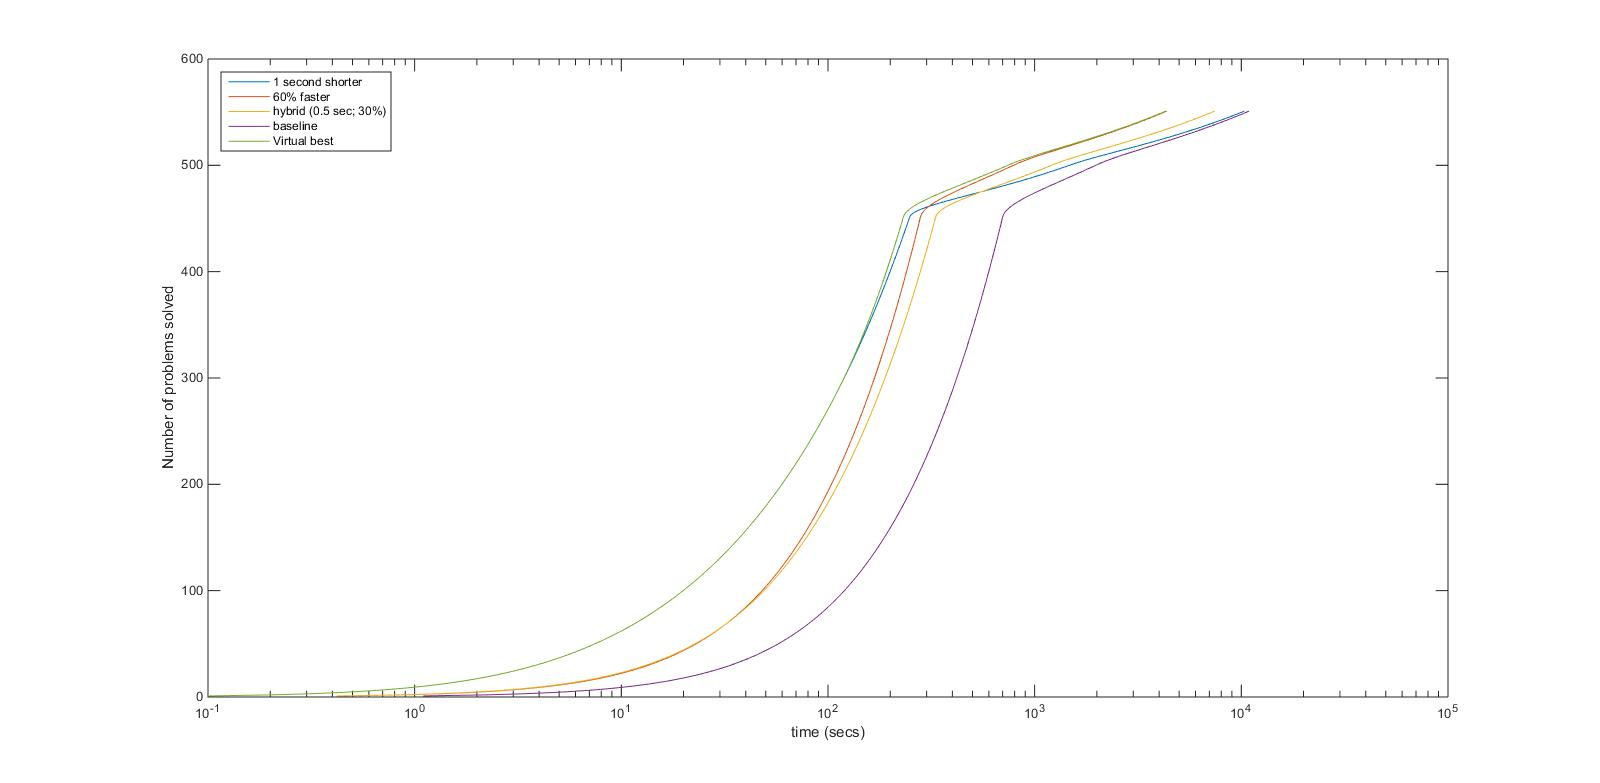
\includegraphics[scale=0.35]{Fig2b.jpg}}
\end{figure}
\clearpage
\section{Case Studies}
%\ednote{Alberto asked ``what's the point''? Good question. I think the first two sections stand as a base case. Then see subsection ``New''.}
For the first three tests we used a vector of baseline times (notionally in seconds) of \\\verb+cat(2,[1.1:0.002:2],[2:1:50],[50:5:300]);+ in MatLab speak, i.e. 1.1 to 2 in steps of 0.002, 2 to 50 in step of 1, and 50 to 300 in steps of 5. 
\subsection{Predictable}\label{sec:Pr}
We first measure four solvers: baseline, baseline less 1 second, 40\% of baseline and a hybrid of 70\% of (baseline less 0.5 seconds). The results are shown in Figure \ref{Fig:S2}. ``1 second shorter'' was quickest 284 times, and ``60\% faster'' 267 times. However, ``60\% faster'' took 48.3 seconds longer than the Virtual Best (which took 4311 seconds),``1 second shorter'' 6036 seconds longer, hybrid  3125 seconds longer and the baseline 6572 seconds longer.
\subsection{Predictable plus Fuzz}\label{sec:P+f}
\begin{figure}[h]
\caption{Data from Section \ref{sec:P+f}\label{Fig:S3}}
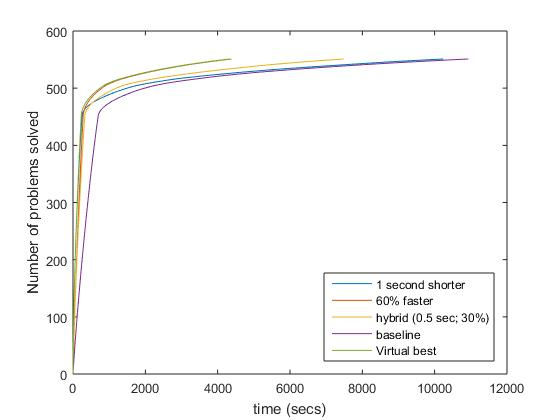
\includegraphics[scale=0.60]{Fig3a.jpg}
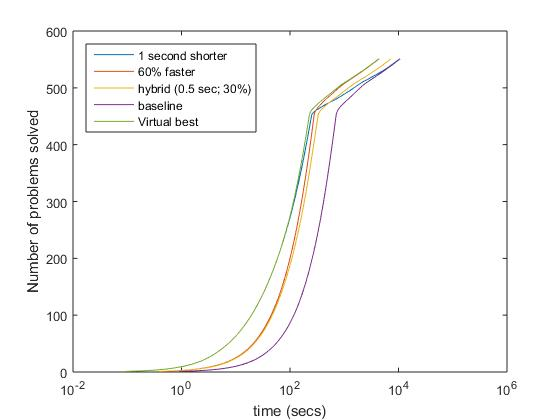
\includegraphics[scale=0.60]{Fig3b.jpg}
\end{figure}
What happens if we multiply each time by a random variable, uniform in [0.8,1.2]? 
%``1 second faster'' was quickest 292 times, hybrid 8 times and ``60\% faster'' 251 times.
40 runs of this experiment give a mean VBS time of 4299 seconds, with a standard deviation of 53.455. In the counts of how often each solver was VBS, hybrid appeared, showing up between 5 and 17 times, with corresponding adjustments to the others. ``1 second shorter'' was always the most common, with the ratio of it over ``60\% faster'' ranging from 1.09 to 1.34. The plots (linear and semilogx) are in Figure \ref{Fig:S3}.
\subsection{Predictable plus Random}\label{sec:P+J}
\begin{figure}[h]
\caption{Data from Section \ref{sec:P+J}\label{Fig:S4}}
\hbox{\hskip-60pt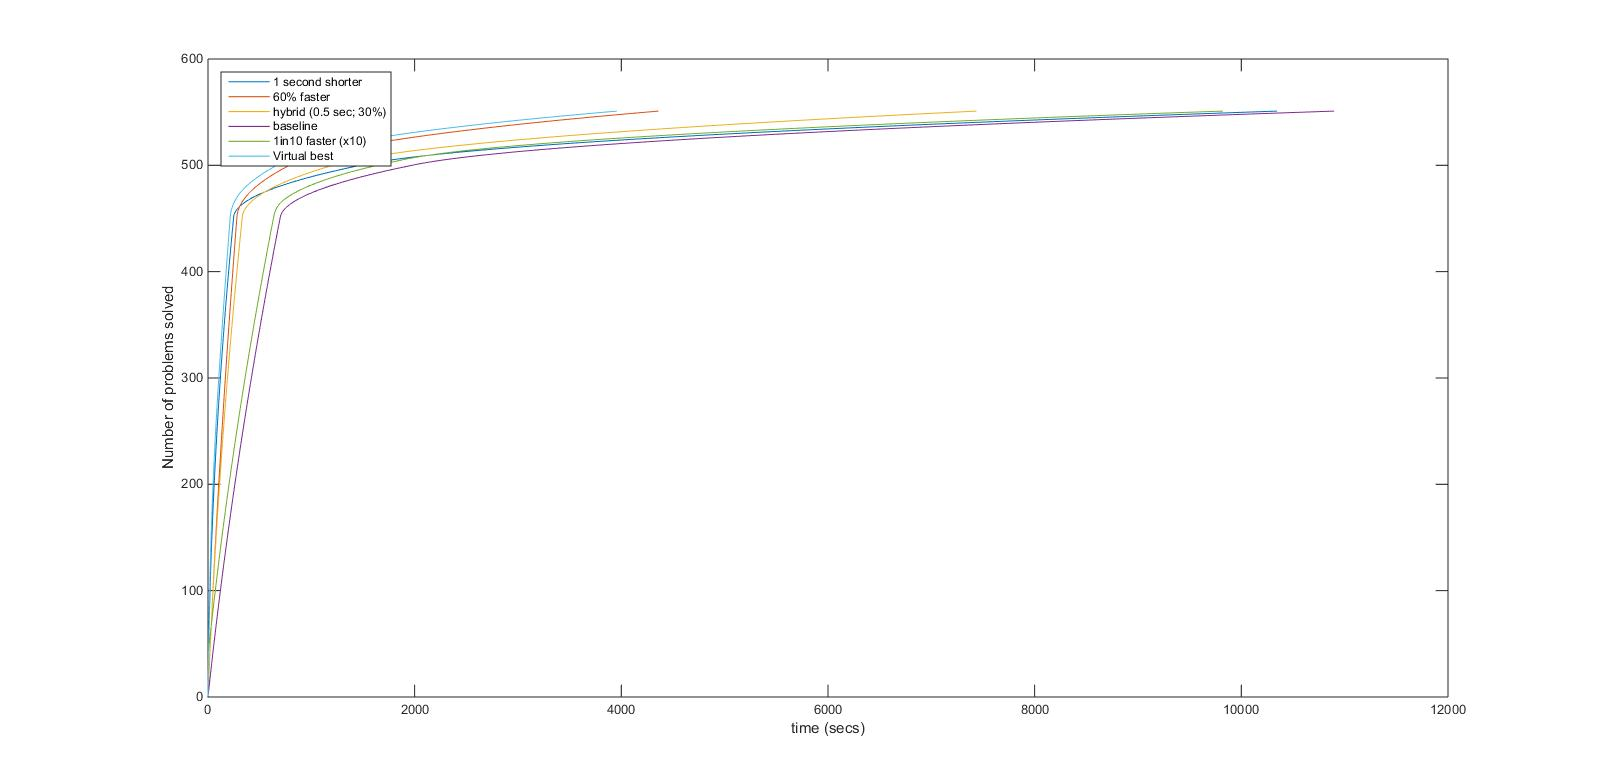
\includegraphics[scale=0.35]{Fig4a.jpg}}
\hbox{\hskip-60pt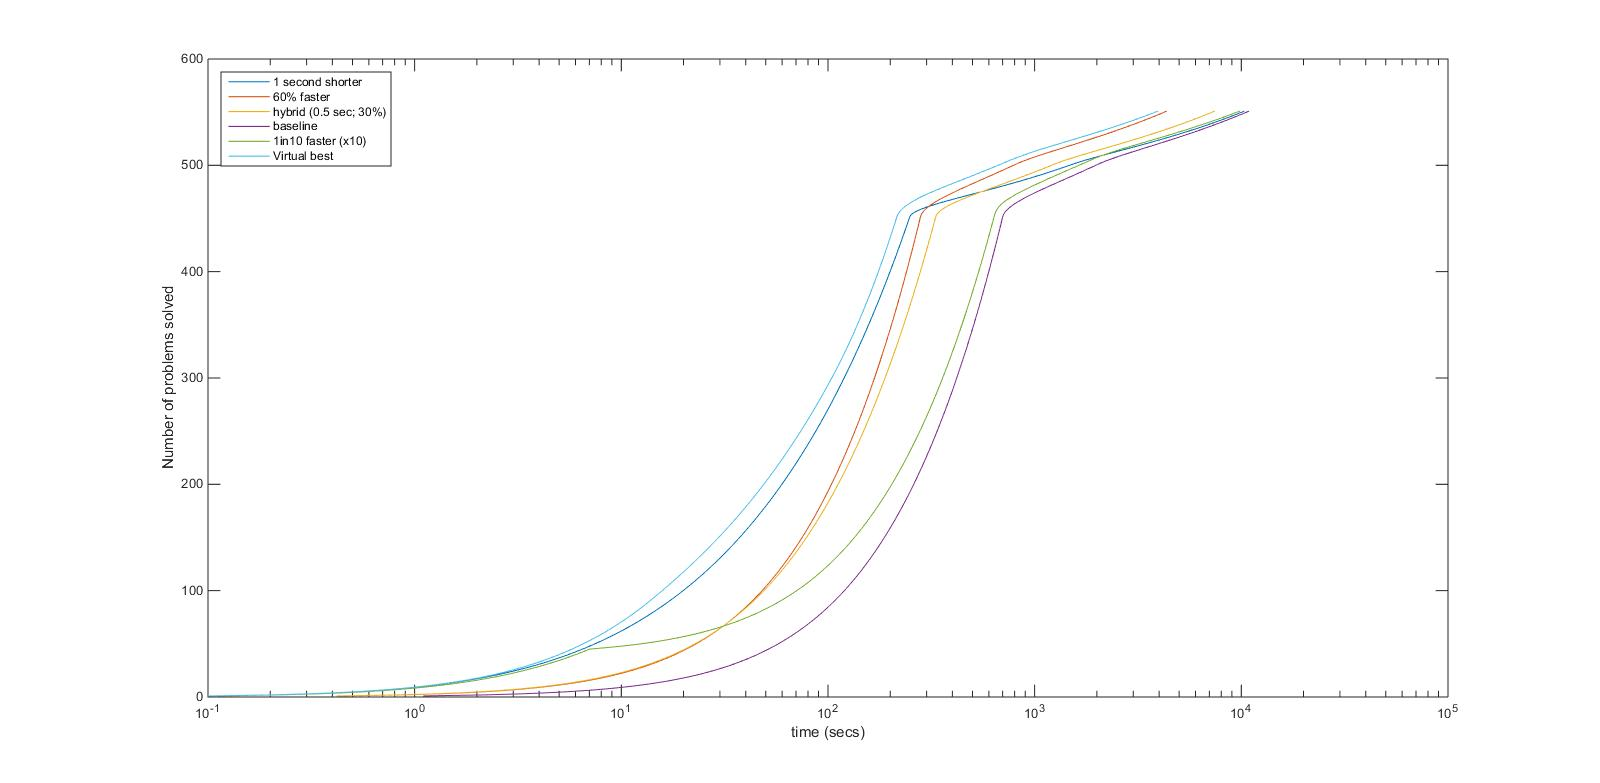
\includegraphics[scale=0.35]{Fig4b.jpg}}
\end{figure}
To the previous solvers, we add a ``joker'', that, on one problem in 10, takes 10\% as long as the baseline.  The results are shown in Figure \ref{Fig:S4}. The joker was quickest 55 times, ``1 second shorter'' was quickest 256 times, and ``60\% faster'' 240 times. The time differences are that ``60\% faster'' took 402 seconds longer than the Virtual Best, ``1 second shorter''  6390 seconds, hybrid 3479 seconds, the joker 5865 seconds and the baseline 6941 seconds.
\subsection{Judgement}\label{sec:J}
\begin{figure}[h]
\caption{Data from Section \ref{sec:J}\label{Fig:S5}}
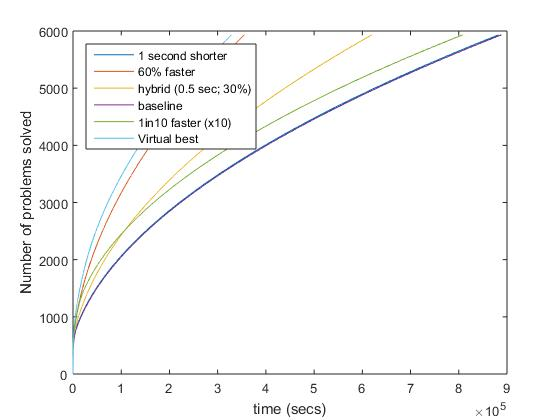
\includegraphics[scale=0.60]{Fig5a.jpg}
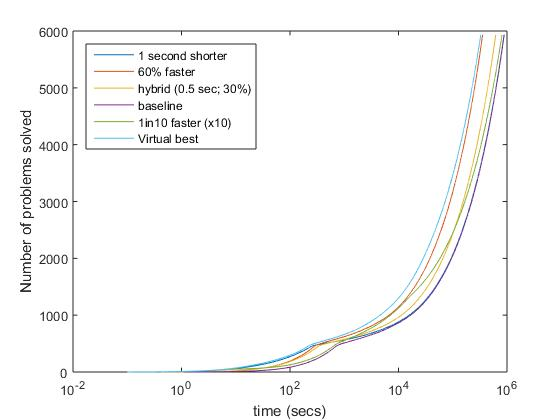
\includegraphics[scale=0.60]{Fig5b.jpg}
\end{figure}
The data used so far had 500 ``fast'' problems ($<2$ seconds), 50 ``medium''  (between 2 and 50) and 5 hard (over 50). What happens if, instead, we have equal numbers in each bracket. The results from this, otherwise using the same methodology as section \ref{sec:P+J}, are in Figure \ref{Fig:S5}: the reader can see the difference from Figure \ref{Fig:S4}: the current figure is dominated by the slow problems. The joker was quickest 593 times, ``1 second shorter'' was quickest 256 times, and ``60\% faster'' 5084 times.
%\subsection{Predictable}
%\section{Martin Brain adds}
\begin{figure}[t]
\vbox{\centering\vskip-100pt
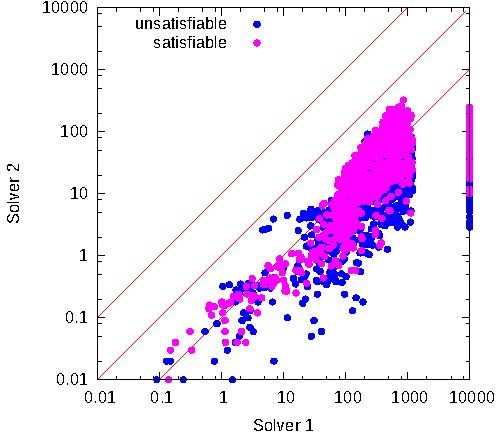
\includegraphics[scale=1.6]{scatter.pdf}}
\caption{Scatter Plot Example.\label{Fig:scatter}}
\end{figure}
\section{Pairwise comparisons}
%\begin{enumerate}
%\item
%The SAT competition has taken to including a "virtual best solver"
%which is synthesised from the other results by taking the minimum (across all solvers tested) time taken to solve every given benchmark.
%Thus the VBS is always equal to the time of some solver, but which one will change by the benchmark (measuring how often each solver is the VBS is also an %interesting metric).  The VBS can be added to the cactus plot to get a feeling for the variability between solvers.
%\item
Scatter plots are used to compare pairs of solvers.  For each benchmark you plot (sometimes using different colours or marks for SAT and UNSAT) a point with x location the time taken by solver 1 and y the time taken by solver 2.  To make things easier to follow, people commonly add the diagonal (sometimes annotated with "solver 1 is faster"
and "solver 2 is faster" on the relevant sides / corners) and the time-out lines.
An example is shown in Figure \ref{Fig:scatter}, from which one might reasonably conclude that Solver 1 is typically 10 times slower than Solver 2, and that Solver 2 never timed out, whereas Solver 1 sometimes did.  loglog plots are usually used, since ratios are the usual deduction. 
\section{Real Life}\label{sec:RL}
This section is drawn from Florian Schanda's joint work with Martin Brain, and the authors are very grateful to him for permission to include the slides.  Figure \ref{CVC16} is a standard tabular presentation of the summary numerical data from his benchmarking. From this one can certainly deduce that Z3 is slightly more  often the winner in terms of \%age of problems solved in each category. 
On the Schanda set (Figure \ref{CVC21}), Z3 is the winner, but Colibri is faster while it's in the race. The virtual best solver has a surprisingly good performance, remaining almost flat much longer than Colibri, and solving significantly more than any individual solver.
\par
 Nevertheless, Z3 is not a winner on the Griggio set, and this is clearly shown in Figure \ref{CVC22}. Also shown here is the fact the the Virtual Best Solver, while tracking Colibri closely, solves a few more. 
%However, the data are not always so clear: consider Heizmann. Here Figure \ref{CVC16} tells is that Z3 comes third, beating MATHSAT(ACDL). However, a look at Figure  \ref{CVC23} shows that it's not so clear: yes, Z3 ultimately solves more, but takes a lot longer doing it.
\begin{figure}[h]
\caption{Numerical Data for ``Real Life''\label{CVC16}}
\vskip-160pt
{\hskip-180pt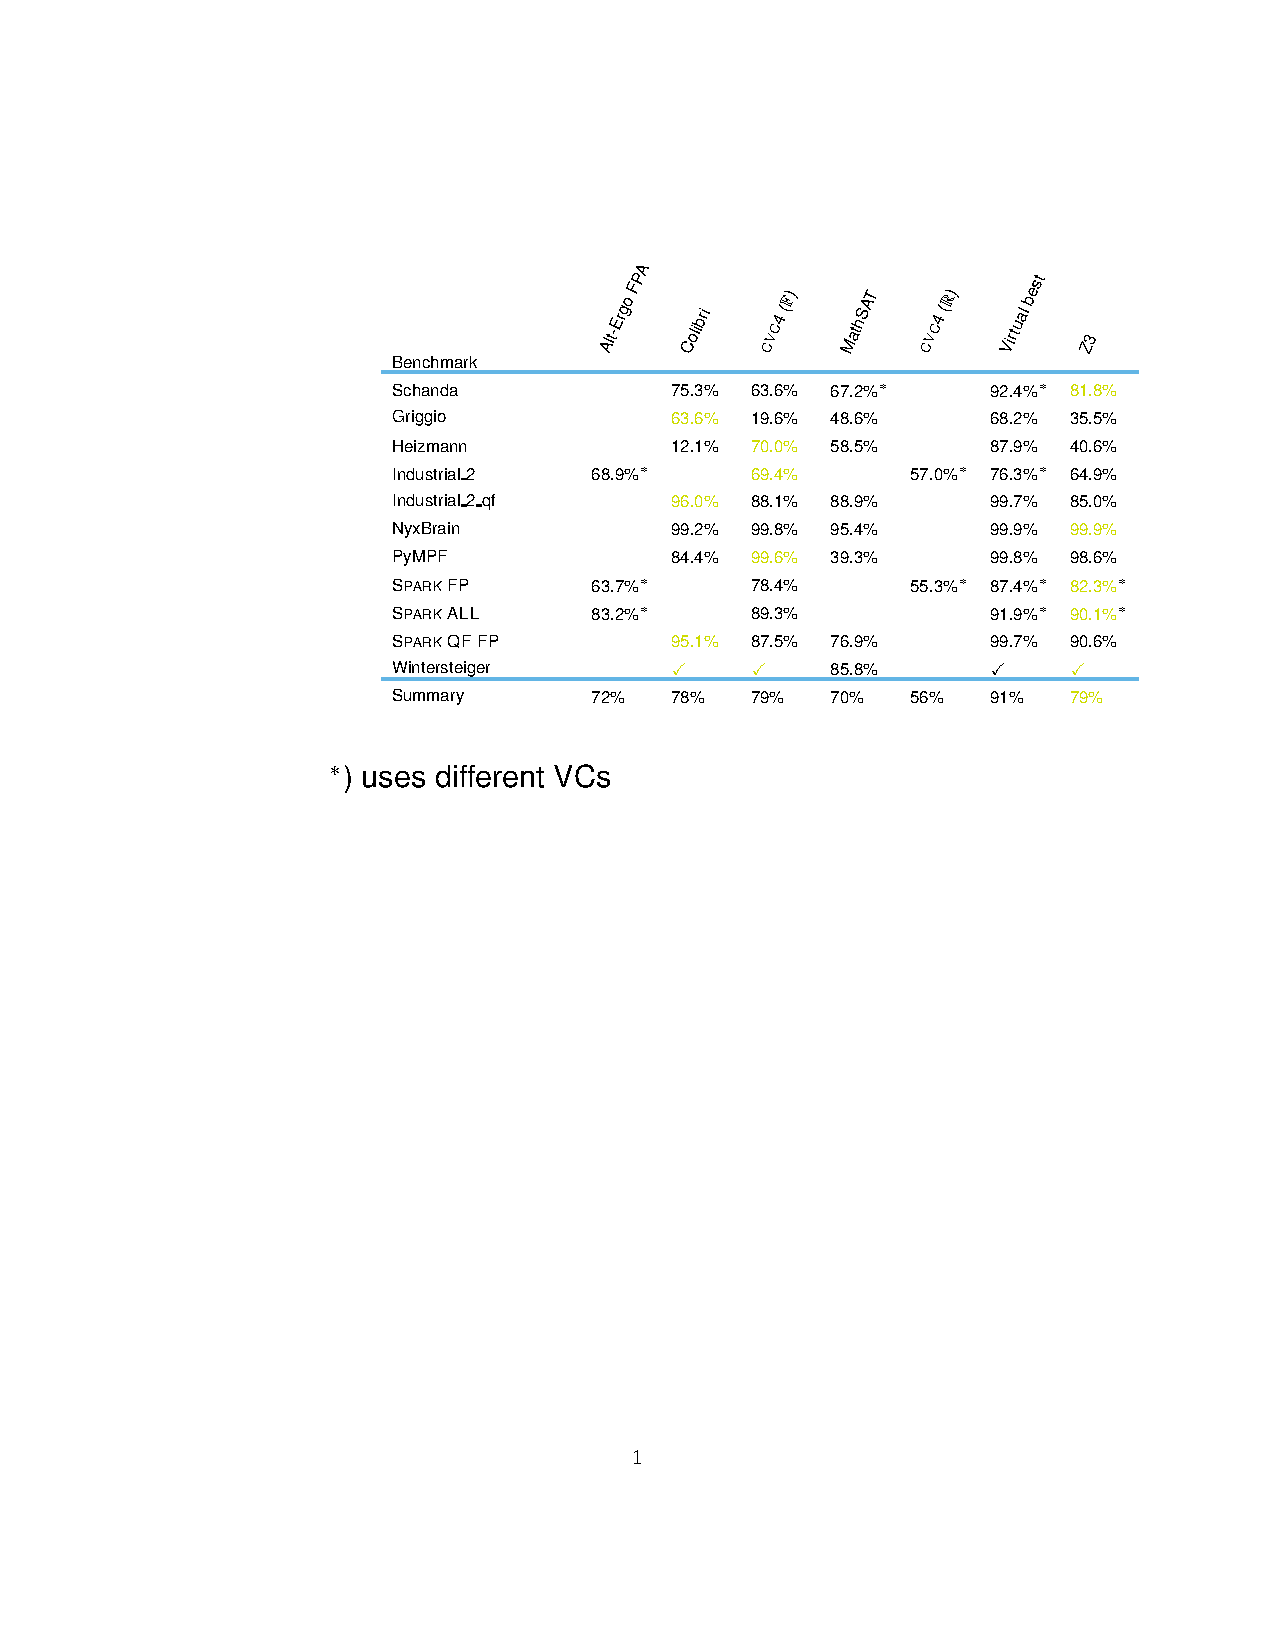
\includegraphics{ExtractCVC16trimv2.pdf}}\vskip-200pt
\end{figure}\iffalse
\begin{figure}[h]
\caption{Numerical Data v2\label{CVC16}}
\begin{center}
\begin{tikzpicture}
\node[anchor=west] at (0.000, 0.000) {\tiny Benchmark};
\node[anchor=west,rotate=65] at (2.750, 0.000) {\tiny Alt-Ergo FPA};
\node[anchor=west,rotate=65] at (3.750, 0.000) {\tiny Colibri};
\node[anchor=west,rotate=65] at (4.750, 0.000) {\tiny {\sc cvc4} (${\mathbb F}$)};
\node[anchor=west,rotate=65] at (5.750, 0.000) {\tiny MathSAT};
\node[anchor=west,rotate=65] at (6.750, 0.000) {\tiny {\sc cvc4} (${\mathbb R}$)};
\node[anchor=west,rotate=65] at (7.750, 0.000) {\tiny Virtual best};
\node[anchor=west,rotate=65] at (8.750, 0.000) {\tiny Z3};
\draw[Altran2,thick] (0.000, -0.125) -- (9.500, -0.125);
\node[anchor=west] at (0.000, -0.350) {\tiny Schanda};
\node[anchor=west] at (7.500, -0.350) {\tiny 92.4\%$^*$};
\node[anchor=west] at (5.500, -0.350) {\tiny 67.2\%$^*$};
\node[anchor=west] at (4.500, -0.350) {\tiny 63.6\%};
\node[anchor=west] at (3.500, -0.350) {\tiny 75.3\%};
\node[anchor=west] at (8.500, -0.350) {\tiny {\color{AnSecondaryGreen}81.8\%}};
\node[anchor=west] at (0.000, -0.700) {\tiny Griggio};
\node[anchor=west] at (7.500, -0.700) {\tiny 68.2\%};
\node[anchor=west] at (5.500, -0.700) {\tiny 48.6\%};
\node[anchor=west] at (4.500, -0.700) {\tiny 19.6\%};
\node[anchor=west] at (3.500, -0.700) {\tiny {\color{AnSecondaryGreen}63.6\%}};
\node[anchor=west] at (8.500, -0.700) {\tiny 35.5\%};
\node[anchor=west] at (0.000, -1.050) {\tiny Heizmann};
\node[anchor=west] at (7.500, -1.050) {\tiny 87.9\%};
\node[anchor=west] at (5.500, -1.050) {\tiny 58.5\%};
\node[anchor=west] at (4.500, -1.050) {\tiny {\color{AnSecondaryGreen}70.0\%}};
\node[anchor=west] at (3.500, -1.050) {\tiny 12.1\%};
\node[anchor=west] at (8.500, -1.050) {\tiny 40.6\%};
\node[anchor=west] at (0.000, -1.400) {\tiny Industrial\_2};
\node[anchor=west] at (7.500, -1.400) {\tiny 76.3\%$^*$};
\node[anchor=west] at (4.500, -1.400) {\tiny {\color{AnSecondaryGreen}69.4\%}};
\node[anchor=west] at (2.500, -1.400) {\tiny 68.9\%$^*$};
\node[anchor=west] at (6.500, -1.400) {\tiny 57.0\%$^*$};
\node[anchor=west] at (8.500, -1.400) {\tiny 64.9\%};
\node[anchor=west] at (0.000, -1.750) {\tiny Industrial\_2\_qf};
\node[anchor=west] at (7.500, -1.750) {\tiny 99.7\%};
\node[anchor=west] at (5.500, -1.750) {\tiny 88.9\%};
\node[anchor=west] at (4.500, -1.750) {\tiny 88.1\%};
\node[anchor=west] at (3.500, -1.750) {\tiny {\color{AnSecondaryGreen}96.0\%}};
\node[anchor=west] at (8.500, -1.750) {\tiny 85.0\%};
\node[anchor=west] at (0.000, -2.100) {\tiny NyxBrain};
\node[anchor=west] at (7.500, -2.100) {\tiny 99.9\%};
\node[anchor=west] at (5.500, -2.100) {\tiny 95.4\%};
\node[anchor=west] at (4.500, -2.100) {\tiny 99.8\%};
\node[anchor=west] at (3.500, -2.100) {\tiny 99.2\%};
\node[anchor=west] at (8.500, -2.100) {\tiny {\color{AnSecondaryGreen}99.9\%}};
\node[anchor=west] at (0.000, -2.450) {\tiny PyMPF};
\node[anchor=west] at (7.500, -2.450) {\tiny 99.8\%};
\node[anchor=west] at (5.500, -2.450) {\tiny 39.3\%};
\node[anchor=west] at (4.500, -2.450) {\tiny {\color{AnSecondaryGreen}99.6\%}};
\node[anchor=west] at (3.500, -2.450) {\tiny 84.4\%};
\node[anchor=west] at (8.500, -2.450) {\tiny 98.6\%};
\node[anchor=west] at (0.000, -2.800) {\tiny {\sc Spark~FP}};
\node[anchor=west] at (7.500, -2.800) {\tiny 87.4\%$^*$};
\node[anchor=west] at (4.500, -2.800) {\tiny 78.4\%};
\node[anchor=west] at (2.500, -2.800) {\tiny 63.7\%$^*$};
\node[anchor=west] at (6.500, -2.800) {\tiny 55.3\%$^*$};
\node[anchor=west] at (8.500, -2.800) {\tiny {\color{AnSecondaryGreen}82.3\%}$^*$};
\node[anchor=west] at (0.000, -3.150) {\tiny {\sc Spark~ALL}};
\node[anchor=west] at (7.500, -3.150) {\tiny 91.9\%$^*$};
\node[anchor=west] at (4.500, -3.150) {\tiny 89.3\%};
\node[anchor=west] at (2.500, -3.150) {\tiny 83.2\%$^*$};
\node[anchor=west] at (8.500, -3.150) {\tiny {\color{AnSecondaryGreen}90.1\%}$^*$};
\node[anchor=west] at (0.000, -3.500) {\tiny {\sc Spark~QF~FP}};
\node[anchor=west] at (7.500, -3.500) {\tiny 99.7\%};
\node[anchor=west] at (5.500, -3.500) {\tiny 76.9\%};
\node[anchor=west] at (4.500, -3.500) {\tiny 87.5\%};
\node[anchor=west] at (3.500, -3.500) {\tiny {\color{AnSecondaryGreen}95.1\%}};
\node[anchor=west] at (8.500, -3.500) {\tiny 90.6\%};
\node[anchor=west] at (0.000, -3.850) {\tiny Wintersteiger};
\node[anchor=west] at (7.500, -3.850) {\tiny $\checkmark$};
\node[anchor=west] at (5.500, -3.850) {\tiny 85.8\%};
\node[anchor=west] at (4.500, -3.850) {\tiny {\color{AnSecondaryGreen}$\checkmark$}};
\node[anchor=west] at (3.500, -3.850) {\tiny {\color{AnSecondaryGreen}$\checkmark$}};
\node[anchor=west] at (8.500, -3.850) {\tiny {\color{AnSecondaryGreen}$\checkmark$}};
\draw[Altran2,thick] (0.000, -3.975) -- (9.500, -3.975);
\node[anchor=west] at (0.000, -4.200) {\tiny Summary};
\node[anchor=west] at (3.500, -4.200) {\tiny 78\%};
\node[anchor=west] at (4.500, -4.200) {\tiny 79\%};
\node[anchor=west] at (6.500, -4.200) {\tiny 56\%};
\node[anchor=west] at (2.500, -4.200) {\tiny 72\%};
\node[anchor=west] at (7.500, -4.200) {\tiny 91\%};
\node[anchor=west] at (5.500, -4.200) {\tiny 70\%};
\node[anchor=west] at (8.500, -4.200) {\tiny {\color{AnSecondaryGreen}79\%}};
\end{tikzpicture}
\end{center}
$^*$) uses different VCs
\end{figure}\fi
\begin{figure}[h]
\caption{Schanda Cactus Plot\label{CVC21}}\begin{center}
\begin{tikzpicture}
\datavisualization [
  scientific axes=clean,
  x axis={
    length=6cm,
    label={instances solved},
    include value=198.00,
    },
  y axis={
    length=6cm,
    label={time},
    ticks={tick unit=s},
  },
  visualize as smooth line=sol5,
  visualize as line=sol1,
  visualize as line=sol2,
  visualize as line=sol3,
  visualize as line=sol6,
  legend={right},
  sol5={label in legend={text=Virtual best},style={dashed}},
  sol1={label in legend={text=Colibri}},
  sol2={label in legend={text={\sc cvc4} (${\mathbb F}$)}},
  sol3={label in legend={text=MathSAT}},
  sol6={label in legend={text=Z3}},
  style sheet=altran
]
data [set=sol5] {
  x, y
  16.00, 0.00
  24.00, 0.01
  53.00, 0.02
  61.00, 0.03
  73.00, 0.04
  77.00, 0.05
  81.00, 0.06
  87.00, 0.07
  88.00, 0.08
  89.00, 0.09
  93.00, 0.10
  95.00, 0.12
  97.00, 0.13
  99.00, 0.14
  100.00, 0.15
  102.00, 0.16
  105.00, 0.18
  106.00, 0.20
  108.00, 0.22
  110.00, 0.23
  116.00, 0.24
  123.00, 0.25
  130.00, 0.26
  143.00, 0.27
  152.00, 0.28
  156.00, 0.29
  157.00, 0.30
  158.00, 0.31
  159.00, 0.32
  160.00, 0.39
  161.00, 0.40
  163.00, 0.43
  164.00, 0.44
  165.00, 0.56
  166.00, 0.58
  167.00, 0.71
  168.00, 0.72
  169.00, 0.82
  170.00, 0.90
  171.00, 1.78
  172.00, 1.79
  173.00, 2.19
  174.00, 2.87
  175.00, 3.04
  176.00, 3.69
  177.00, 3.90
  178.00, 4.88
  179.00, 8.57
  180.00, 12.86
  181.00, 14.21
  182.00, 16.34
  183.00, 20.69
}
data [set=sol1] {
  x, y
  2.00, 0.22
  7.00, 0.23
  15.00, 0.24
  31.00, 0.25
  71.00, 0.26
  108.00, 0.27
  134.00, 0.28
  139.00, 0.29
  140.00, 0.30
  141.00, 0.31
  143.00, 0.32
  144.00, 0.35
  145.00, 0.58
  146.00, 0.61
  147.00, 0.90
  148.00, 1.16
  149.00, 4.88
}
data [set=sol2] {
  x, y
  16.00, 0.00
  23.00, 0.01
  35.00, 0.02
  45.00, 0.03
  56.00, 0.04
  58.00, 0.05
  61.00, 0.06
  64.00, 0.07
  68.00, 0.08
  69.00, 0.09
  73.00, 0.10
  74.00, 0.11
  77.00, 0.12
  78.00, 0.13
  79.00, 0.14
  80.00, 0.16
  81.00, 0.17
  82.00, 0.24
  83.00, 0.26
  84.00, 0.29
  85.00, 0.32
  86.00, 0.34
  88.00, 0.36
  89.00, 0.38
  90.00, 0.40
  91.00, 0.41
  93.00, 0.42
  94.00, 0.43
  95.00, 0.44
  96.00, 0.51
  97.00, 0.54
  98.00, 0.59
  100.00, 0.70
  101.00, 0.71
  102.00, 0.78
  103.00, 0.81
  104.00, 0.84
  105.00, 0.99
  106.00, 1.08
  107.00, 1.26
  108.00, 1.52
  109.00, 1.55
  110.00, 1.60
  111.00, 1.73
  112.00, 2.13
  113.00, 2.19
  114.00, 2.29
  115.00, 2.68
  116.00, 3.20
  117.00, 5.37
  118.00, 6.22
  119.00, 10.20
  120.00, 11.80
  121.00, 12.56
  122.00, 13.06
  123.00, 14.03
  124.00, 16.52
  125.00, 17.06
  126.00, 24.67
}
data [set=sol3] {
  x, y
  4.00, 0.00
  12.00, 0.01
  43.00, 0.02
  51.00, 0.03
  55.00, 0.04
  57.00, 0.05
  61.00, 0.06
  66.00, 0.07
  68.00, 0.08
  70.00, 0.10
  71.00, 0.11
  72.00, 0.12
  75.00, 0.13
  78.00, 0.14
  79.00, 0.15
  83.00, 0.18
  85.00, 0.20
  86.00, 0.22
  88.00, 0.24
  89.00, 0.28
  90.00, 0.29
  91.00, 0.31
  92.00, 0.35
  93.00, 0.38
  95.00, 0.39
  96.00, 0.41
  97.00, 0.43
  98.00, 0.44
  99.00, 0.46
  100.00, 0.49
  101.00, 0.51
  102.00, 0.52
  104.00, 0.56
  105.00, 0.59
  106.00, 0.60
  107.00, 0.62
  108.00, 0.74
  109.00, 0.79
  110.00, 0.82
  111.00, 0.83
  112.00, 0.88
  113.00, 0.89
  114.00, 0.92
  115.00, 1.07
  116.00, 1.67
  117.00, 1.79
  118.00, 2.15
  119.00, 2.22
  120.00, 2.25
  121.00, 2.81
  122.00, 3.65
  123.00, 3.69
  124.00, 6.12
  125.00, 7.03
  126.00, 7.46
  127.00, 8.76
  128.00, 9.31
  129.00, 10.87
  130.00, 13.82
  131.00, 17.58
  132.00, 29.03
  133.00, 51.90
}
data [set=sol6] {
  x, y
  18.00, 0.04
  55.00, 0.05
  61.00, 0.06
  72.00, 0.07
  73.00, 0.09
  75.00, 0.12
  77.00, 0.14
  78.00, 0.16
  81.00, 0.18
  82.00, 0.20
  83.00, 0.21
  85.00, 0.22
  86.00, 0.25
  89.00, 0.26
  91.00, 0.27
  92.00, 0.30
  93.00, 0.34
  94.00, 0.38
  96.00, 0.40
  98.00, 0.42
  99.00, 0.44
  100.00, 0.46
  101.00, 0.49
  102.00, 0.51
  103.00, 0.56
  104.00, 0.57
  105.00, 0.63
  106.00, 0.66
  107.00, 0.70
  108.00, 0.72
  109.00, 0.83
  110.00, 1.21
  111.00, 1.25
  112.00, 1.32
  113.00, 1.42
  115.00, 1.64
  116.00, 1.74
  117.00, 1.78
  118.00, 1.93
  119.00, 1.95
  120.00, 1.97
  121.00, 2.00
  122.00, 2.02
  123.00, 2.11
  124.00, 2.12
  125.00, 2.19
  126.00, 2.31
  127.00, 2.41
  128.00, 2.42
  129.00, 2.51
  130.00, 2.54
  131.00, 2.58
  132.00, 2.62
  133.00, 2.87
  134.00, 2.94
  135.00, 2.97
  136.00, 3.03
  137.00, 3.04
  138.00, 3.15
  139.00, 3.26
  140.00, 3.64
  141.00, 3.69
  142.00, 3.90
  143.00, 4.18
  144.00, 5.17
  145.00, 5.27
  146.00, 6.36
  147.00, 7.47
  148.00, 8.34
  149.00, 8.57
  150.00, 11.44
  151.00, 12.46
  152.00, 12.86
  153.00, 13.28
  154.00, 14.21
  155.00, 14.96
  156.00, 16.34
  157.00, 17.68
  158.00, 19.30
  159.00, 20.69
  160.00, 35.09
  161.00, 39.24
  162.00, 49.26
}
;
\end{tikzpicture}
\end{center}
\end{figure}
\begin{figure}[h]
\caption{Griggio Cactus Plot\label{CVC22}}
\begin{center}
\begin{tikzpicture}
\datavisualization [
  scientific axes=clean,
  x axis={
    length=6cm,
    label={instances solved},
    include value=214.00,
    },
  y axis={
    length=6cm,
    label={time},
    ticks={tick unit=s},
  },
  visualize as smooth line=sol5,
  visualize as line=sol1,
  visualize as line=sol2,
  visualize as line=sol3,
  visualize as line=sol6,
  legend={right},
  sol5={label in legend={text=Virtual best},style={dashed}},
  sol1={label in legend={text=Colibri}},
  sol2={label in legend={text={\sc cvc4} (${\mathbb F}$)}},
  sol3={label in legend={text=MathSAT}},
  sol6={label in legend={text=Z3}},
  style sheet=altran
]
data [set=sol5] {
  x, y
  2.00, 0.00
  4.00, 0.01
  6.00, 0.02
  8.00, 0.12
  9.00, 0.13
  10.00, 0.14
  11.00, 0.15
  14.00, 0.16
  15.00, 0.22
  17.00, 0.26
  19.00, 0.27
  20.00, 0.28
  21.00, 0.29
  24.00, 0.30
  29.00, 0.31
  38.00, 0.32
  40.00, 0.33
  42.00, 0.34
  47.00, 0.35
  60.00, 0.36
  61.00, 0.37
  64.00, 0.38
  66.00, 0.39
  68.00, 0.40
  69.00, 0.42
  71.00, 0.44
  73.00, 0.45
  75.00, 0.46
  76.00, 0.53
  78.00, 0.54
  79.00, 0.55
  80.00, 0.56
  81.00, 0.58
  82.00, 0.59
  83.00, 0.60
  84.00, 0.66
  85.00, 0.69
  86.00, 0.72
  87.00, 0.74
  88.00, 0.77
  89.00, 0.80
  90.00, 0.86
  91.00, 0.88
  92.00, 0.92
  93.00, 0.97
  94.00, 1.13
  95.00, 1.19
  96.00, 1.36
  97.00, 1.39
  98.00, 1.42
  99.00, 1.48
  100.00, 1.60
  101.00, 1.62
  102.00, 1.66
  103.00, 1.69
  104.00, 1.79
  105.00, 1.83
  106.00, 1.97
  107.00, 2.03
  108.00, 2.11
  109.00, 2.18
  110.00, 2.41
  111.00, 2.52
  112.00, 2.69
  113.00, 3.03
  114.00, 3.06
  115.00, 3.13
  116.00, 3.19
  117.00, 3.66
  118.00, 3.82
  119.00, 3.89
  120.00, 3.90
  121.00, 3.93
  122.00, 4.51
  123.00, 4.77
  124.00, 4.78
  125.00, 6.28
  126.00, 6.32
  127.00, 6.92
  128.00, 7.15
  129.00, 8.14
  130.00, 9.16
  131.00, 12.55
  132.00, 12.66
  133.00, 12.81
  134.00, 12.94
  135.00, 16.12
  136.00, 16.23
  137.00, 18.04
  138.00, 20.56
  139.00, 24.63
  140.00, 27.01
  141.00, 35.11
  142.00, 36.33
  143.00, 36.43
  144.00, 36.87
  145.00, 52.58
  146.00, 58.00
}
data [set=sol1] {
  x, y
  2.00, 0.26
  5.00, 0.27
  9.00, 0.28
  13.00, 0.29
  18.00, 0.30
  23.00, 0.31
  33.00, 0.32
  36.00, 0.33
  38.00, 0.34
  43.00, 0.35
  56.00, 0.36
  57.00, 0.37
  60.00, 0.38
  62.00, 0.39
  64.00, 0.40
  65.00, 0.42
  67.00, 0.44
  69.00, 0.45
  71.00, 0.46
  72.00, 0.53
  74.00, 0.54
  75.00, 0.55
  76.00, 0.56
  77.00, 0.58
  78.00, 0.59
  79.00, 0.60
  80.00, 0.66
  81.00, 0.69
  82.00, 0.72
  83.00, 0.74
  84.00, 0.80
  85.00, 0.86
  86.00, 0.92
  87.00, 0.97
  88.00, 1.13
  89.00, 1.19
  90.00, 1.30
  91.00, 1.36
  92.00, 1.39
  93.00, 1.42
  94.00, 1.48
  95.00, 1.60
  96.00, 1.62
  97.00, 1.66
  98.00, 1.69
  99.00, 1.79
  100.00, 1.83
  101.00, 1.97
  102.00, 2.03
  103.00, 2.11
  104.00, 2.18
  105.00, 2.41
  106.00, 2.52
  107.00, 2.69
  108.00, 3.03
  109.00, 3.06
  110.00, 3.13
  111.00, 3.19
  112.00, 3.66
  113.00, 3.74
  114.00, 3.82
  115.00, 3.89
  116.00, 3.90
  117.00, 3.93
  118.00, 4.48
  119.00, 4.51
  120.00, 4.77
  121.00, 4.78
  122.00, 6.28
  123.00, 6.32
  124.00, 6.92
  125.00, 7.15
  126.00, 8.12
  127.00, 8.14
  128.00, 8.34
  129.00, 9.16
  130.00, 12.66
  131.00, 12.81
  132.00, 12.94
  133.00, 16.12
  134.00, 27.01
  135.00, 36.43
  136.00, 43.33
}
data [set=sol2] {
  x, y
  1.00, 0.00
  2.00, 0.04
  3.00, 0.17
  4.00, 0.26
  5.00, 0.44
  6.00, 0.54
  7.00, 0.63
  9.00, 0.65
  10.00, 0.67
  11.00, 0.77
  12.00, 0.85
  13.00, 0.88
  14.00, 0.91
  15.00, 1.02
  16.00, 1.32
  18.00, 1.34
  19.00, 1.52
  20.00, 2.37
  21.00, 2.55
  22.00, 2.92
  23.00, 4.65
  24.00, 5.05
  25.00, 6.27
  26.00, 8.23
  27.00, 8.24
  28.00, 8.34
  29.00, 8.37
  31.00, 9.73
  32.00, 9.82
  33.00, 12.34
  34.00, 13.42
  35.00, 15.40
  36.00, 16.34
  37.00, 47.10
  38.00, 50.61
  39.00, 54.37
  40.00, 54.68
  41.00, 54.99
  42.00, 58.00
}
data [set=sol3] {
  x, y
  2.00, 0.00
  4.00, 0.01
  6.00, 0.02
  7.00, 0.12
  8.00, 0.13
  9.00, 0.14
  11.00, 0.15
  14.00, 0.16
  15.00, 0.22
  16.00, 0.27
  17.00, 0.32
  18.00, 0.53
  19.00, 0.88
  20.00, 0.96
  21.00, 1.06
  22.00, 1.12
  23.00, 1.22
  24.00, 1.29
  25.00, 1.46
  26.00, 1.57
  27.00, 1.63
  29.00, 1.71
  31.00, 1.88
  32.00, 2.12
  33.00, 2.18
  34.00, 2.27
  35.00, 2.52
  36.00, 3.01
  37.00, 3.03
  38.00, 4.39
  39.00, 4.62
  40.00, 6.20
  41.00, 7.44
  42.00, 7.46
  43.00, 7.59
  44.00, 7.61
  45.00, 7.98
  46.00, 8.07
  47.00, 8.34
  48.00, 8.64
  49.00, 8.94
  50.00, 9.38
  51.00, 9.56
  52.00, 10.51
  53.00, 10.75
  54.00, 13.42
  55.00, 13.58
  56.00, 13.68
  57.00, 14.54
  58.00, 15.33
  59.00, 16.19
  60.00, 16.23
  61.00, 16.58
  62.00, 16.78
  63.00, 17.34
  64.00, 17.74
  65.00, 18.04
  66.00, 18.93
  67.00, 19.24
  68.00, 20.56
  69.00, 20.58
  70.00, 20.67
  71.00, 22.71
  72.00, 23.41
  73.00, 24.63
  74.00, 25.24
  75.00, 26.33
  76.00, 27.81
  77.00, 28.17
  78.00, 28.20
  79.00, 28.65
  80.00, 28.69
  81.00, 28.78
  82.00, 31.10
  83.00, 31.23
  84.00, 32.17
  85.00, 33.49
  86.00, 35.11
  87.00, 35.58
  88.00, 35.84
  89.00, 36.33
  90.00, 36.59
  91.00, 36.87
  92.00, 37.86
  93.00, 38.03
  94.00, 39.19
  95.00, 39.32
  96.00, 40.14
  97.00, 42.54
  98.00, 42.59
  99.00, 42.97
  100.00, 47.56
  101.00, 48.56
  102.00, 51.01
  103.00, 52.58
  104.00, 55.55
}
data [set=sol6] {
  x, y
  2.00, 0.05
  3.00, 0.12
  4.00, 0.56
  5.00, 0.58
  6.00, 0.62
  7.00, 0.66
  9.00, 0.84
  10.00, 0.90
  11.00, 0.95
  12.00, 0.98
  13.00, 1.24
  14.00, 2.23
  15.00, 2.62
  16.00, 3.62
  17.00, 3.67
  18.00, 3.73
  19.00, 3.91
  20.00, 4.07
  21.00, 4.38
  22.00, 4.48
  23.00, 4.71
  24.00, 5.20
  25.00, 5.25
  26.00, 5.66
  27.00, 5.96
  28.00, 6.02
  29.00, 6.52
  30.00, 6.95
  31.00, 7.43
  32.00, 7.44
  33.00, 7.80
  34.00, 8.30
  35.00, 8.70
  36.00, 9.28
  37.00, 9.60
  38.00, 10.01
  39.00, 10.21
  40.00, 10.24
  41.00, 12.55
  42.00, 12.86
  43.00, 18.20
  44.00, 19.80
  45.00, 19.91
  46.00, 21.65
  47.00, 22.55
  48.00, 23.16
  49.00, 23.88
  50.00, 24.09
  51.00, 24.21
  52.00, 25.89
  53.00, 26.38
  54.00, 26.94
  55.00, 27.03
  56.00, 27.70
  57.00, 29.54
  58.00, 31.79
  59.00, 32.94
  60.00, 33.49
  61.00, 33.61
  62.00, 34.30
  63.00, 37.03
  64.00, 37.44
  65.00, 39.59
  66.00, 41.69
  67.00, 43.96
  68.00, 52.42
  69.00, 52.54
  70.00, 55.11
  71.00, 55.50
  72.00, 56.72
  73.00, 56.85
  74.00, 57.36
  75.00, 58.37
  76.00, 59.80
}
;
\end{tikzpicture}
\end{center}
%\vskip-100pt
%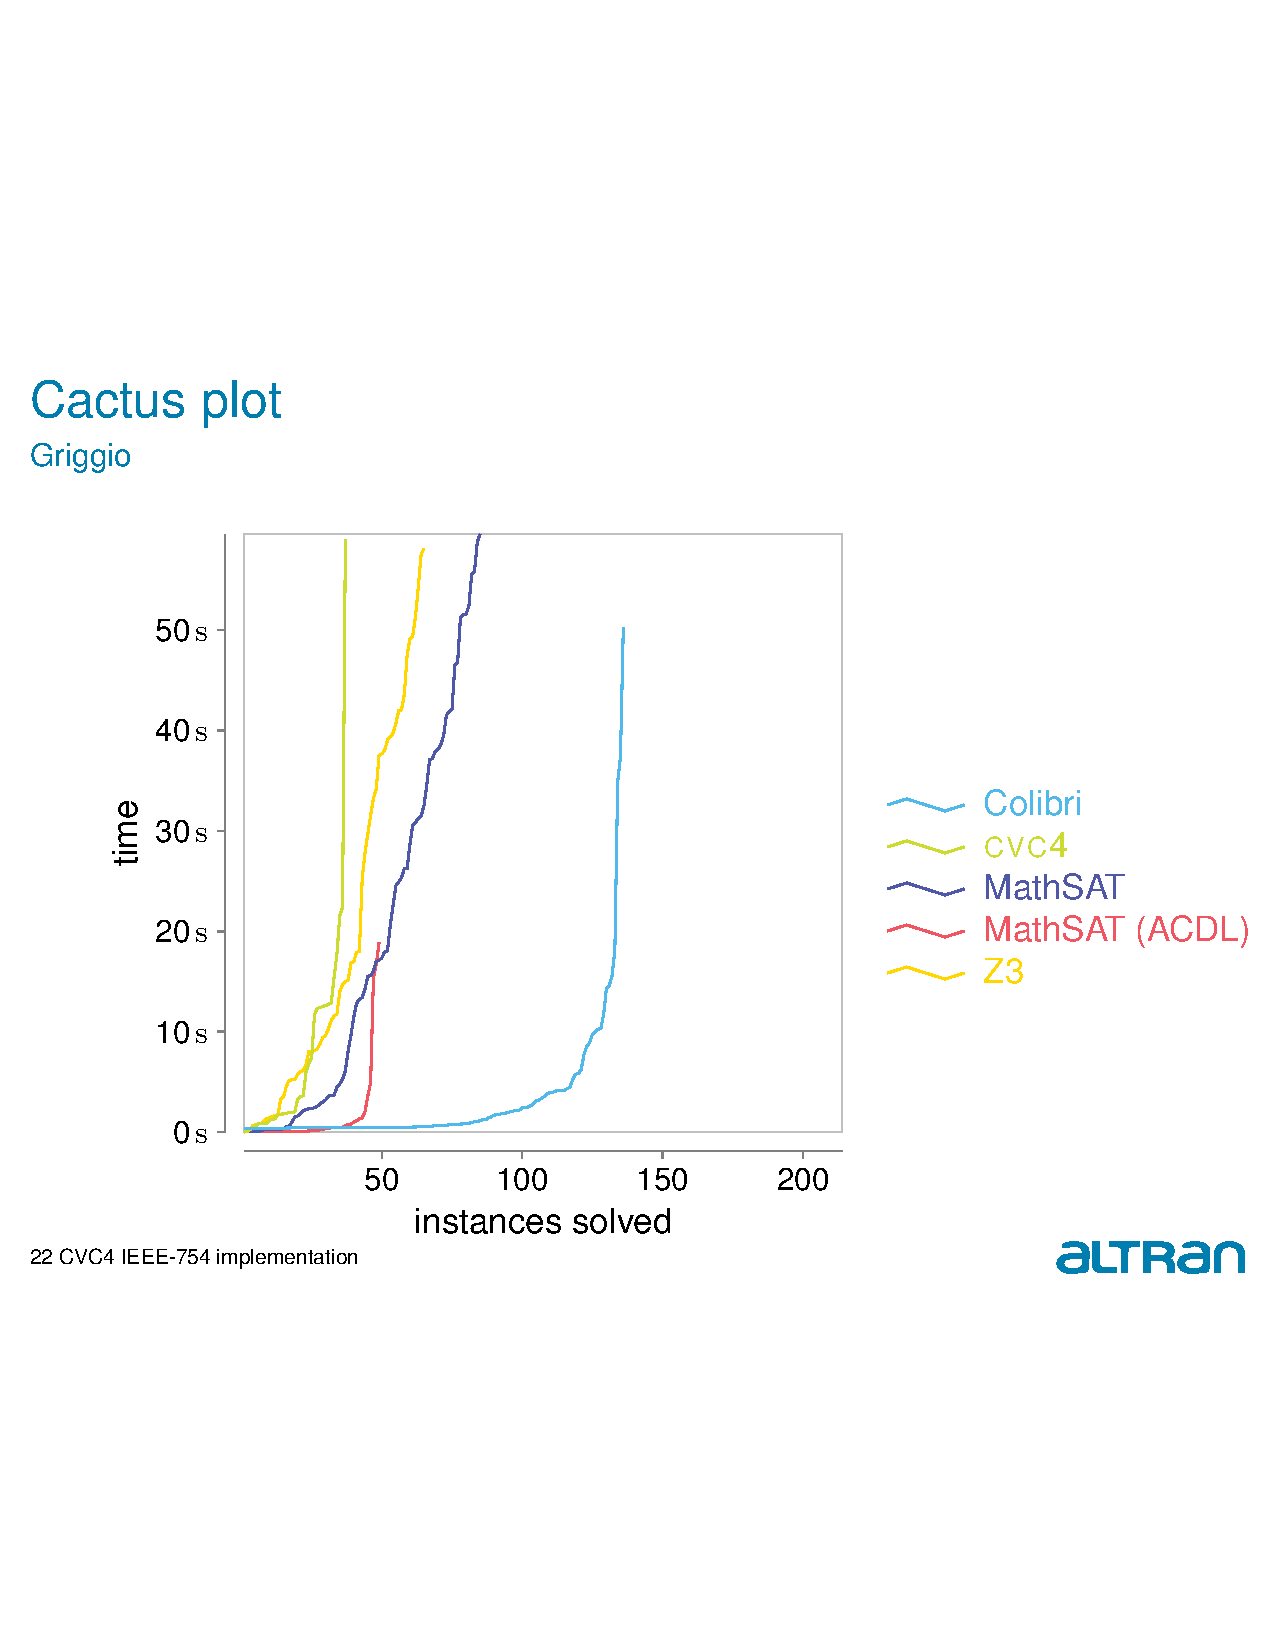
\includegraphics[scale=0.8]{ExtractCVC22.pdf}
\end{figure}\iffalse
\begin{figure}[h]
\caption{Heizmann Cactus Plot\label{CVC23}}
\begin{center}
\begin{tikzpicture}
\datavisualization [
  scientific axes=clean,
  x axis={
    length=6cm,
    label={instances solved},
    include value=207.00,
    },
  y axis={
    length=6cm,
    label={time},
    ticks={tick unit=s},
  },
  visualize as smooth line=sol5,
  visualize as line=sol1,
  visualize as line=sol2,
  visualize as line=sol3,
  visualize as line=sol6,
  legend={right},
  sol5={label in legend={text=Virtual best},style={dashed}},
  sol1={label in legend={text=Colibri}},
  sol2={label in legend={text={\sc cvc4} (${\mathbb F}$)}},
  sol3={label in legend={text=MathSAT}},
  sol6={label in legend={text=Z3}},
  style sheet=altran
]
data [set=sol5] {
  x, y
  12.00, 0.00
  52.00, 0.01
  92.00, 0.02
  98.00, 0.03
  102.00, 0.04
  103.00, 0.06
  104.00, 0.07
  106.00, 0.08
  107.00, 0.10
  108.00, 0.13
  110.00, 0.14
  111.00, 0.16
  112.00, 0.18
  114.00, 0.32
  115.00, 0.46
  116.00, 0.48
  117.00, 0.50
  118.00, 0.53
  119.00, 0.60
  120.00, 0.71
  121.00, 0.72
  123.00, 0.73
  124.00, 0.74
  125.00, 0.79
  126.00, 0.80
  127.00, 0.87
  128.00, 0.88
  129.00, 1.10
  130.00, 1.13
  131.00, 1.19
  132.00, 1.25
  133.00, 1.27
  134.00, 1.44
  135.00, 1.46
  136.00, 1.54
  137.00, 1.57
  138.00, 1.60
  139.00, 1.64
  140.00, 1.67
  141.00, 1.82
  142.00, 1.84
  143.00, 2.25
  144.00, 2.90
  145.00, 2.94
  146.00, 3.02
  147.00, 3.30
  148.00, 3.58
  149.00, 3.64
  150.00, 3.79
  151.00, 4.08
  152.00, 4.51
  153.00, 5.10
  154.00, 5.20
  155.00, 5.36
  156.00, 5.38
  157.00, 5.70
  158.00, 5.86
  159.00, 9.89
  160.00, 11.46
  161.00, 11.49
  162.00, 12.50
  163.00, 14.49
  164.00, 14.65
  165.00, 14.84
  166.00, 15.66
  167.00, 15.94
  168.00, 16.02
  169.00, 16.07
  170.00, 16.49
  171.00, 17.16
  172.00, 17.93
  173.00, 18.00
  174.00, 18.12
  175.00, 18.13
  176.00, 19.02
  177.00, 28.45
  178.00, 34.84
  179.00, 37.30
  180.00, 43.04
  181.00, 43.14
  182.00, 43.82
}
data [set=sol1] {
  x, y
  1.00, 0.26
  2.00, 0.27
  6.00, 0.28
  8.00, 0.29
  9.00, 0.30
  11.00, 0.31
  12.00, 0.32
  15.00, 0.34
  18.00, 0.35
  21.00, 0.36
  22.00, 0.46
  23.00, 0.53
  24.00, 0.71
  25.00, 11.85
}
data [set=sol2] {
  x, y
  5.00, 0.00
  26.00, 0.01
  40.00, 0.02
  49.00, 0.03
  63.00, 0.04
  69.00, 0.05
  85.00, 0.06
  89.00, 0.08
  91.00, 0.09
  97.00, 0.10
  100.00, 0.11
  101.00, 0.12
  102.00, 0.13
  105.00, 0.14
  107.00, 0.15
  109.00, 0.16
  110.00, 0.18
  111.00, 0.32
  112.00, 0.50
  113.00, 0.60
  114.00, 0.72
  117.00, 0.73
  118.00, 0.74
  119.00, 0.86
  120.00, 0.87
  121.00, 0.90
  122.00, 0.93
  123.00, 1.10
  124.00, 1.13
  125.00, 1.19
  126.00, 1.25
  127.00, 1.27
  128.00, 1.44
  129.00, 1.54
  130.00, 1.57
  131.00, 1.60
  132.00, 1.64
  133.00, 1.72
  134.00, 1.82
  135.00, 1.84
  136.00, 2.25
  137.00, 2.90
  138.00, 2.94
  139.00, 3.02
  140.00, 3.30
  141.00, 5.10
  142.00, 12.50
  143.00, 19.88
  144.00, 49.25
  145.00, 49.76
}
data [set=sol3] {
  x, y
  7.00, 0.00
  51.00, 0.01
  91.00, 0.02
  97.00, 0.03
  101.00, 0.04
  102.00, 0.07
  104.00, 0.08
  105.00, 1.30
  106.00, 1.46
  107.00, 3.08
  108.00, 3.58
  109.00, 3.64
  110.00, 3.79
  111.00, 4.08
  112.00, 4.16
  113.00, 4.51
  114.00, 4.79
  115.00, 5.20
  116.00, 5.36
  117.00, 5.38
  118.00, 5.70
  119.00, 5.86
  120.00, 7.16
  121.00, 18.13
}
data [set=sol6] {
  x, y
  1.00, 0.48
  2.00, 0.56
  3.00, 0.61
  4.00, 0.69
  5.00, 0.73
  6.00, 0.79
  7.00, 0.80
  8.00, 0.81
  9.00, 0.87
  10.00, 0.88
  11.00, 1.46
  12.00, 1.67
  13.00, 1.77
  14.00, 2.77
  15.00, 3.34
  16.00, 3.88
  17.00, 3.94
  18.00, 8.06
  19.00, 9.89
  20.00, 10.19
  21.00, 10.23
  22.00, 10.24
  23.00, 10.25
  24.00, 10.29
  25.00, 10.30
  26.00, 11.46
  27.00, 11.49
  28.00, 11.55
  29.00, 12.25
  30.00, 12.40
  31.00, 12.66
  32.00, 12.73
  33.00, 14.40
  34.00, 14.49
  35.00, 14.58
  37.00, 14.65
  38.00, 14.66
  39.00, 14.84
  40.00, 15.15
  41.00, 15.38
  42.00, 15.48
  43.00, 15.66
  44.00, 15.72
  45.00, 15.94
  46.00, 16.02
  47.00, 16.07
  48.00, 16.28
  49.00, 16.49
  50.00, 17.12
  51.00, 17.16
  53.00, 17.44
  54.00, 17.47
  55.00, 17.68
  56.00, 17.93
  57.00, 18.00
  58.00, 18.12
  59.00, 19.02
  60.00, 19.74
  61.00, 20.40
  62.00, 20.44
  63.00, 20.56
  64.00, 20.86
  65.00, 26.00
  66.00, 26.19
  67.00, 26.44
  68.00, 27.32
  69.00, 28.45
  70.00, 29.60
  71.00, 31.93
  72.00, 34.84
  73.00, 37.30
  74.00, 43.04
  75.00, 43.14
  76.00, 43.16
  77.00, 43.82
  78.00, 46.09
  79.00, 49.65
  80.00, 54.18
  81.00, 57.14
  82.00, 58.10
  83.00, 58.41
  84.00, 58.68
}
;
\end{tikzpicture}
\end{center}
%\vskip-100pt
%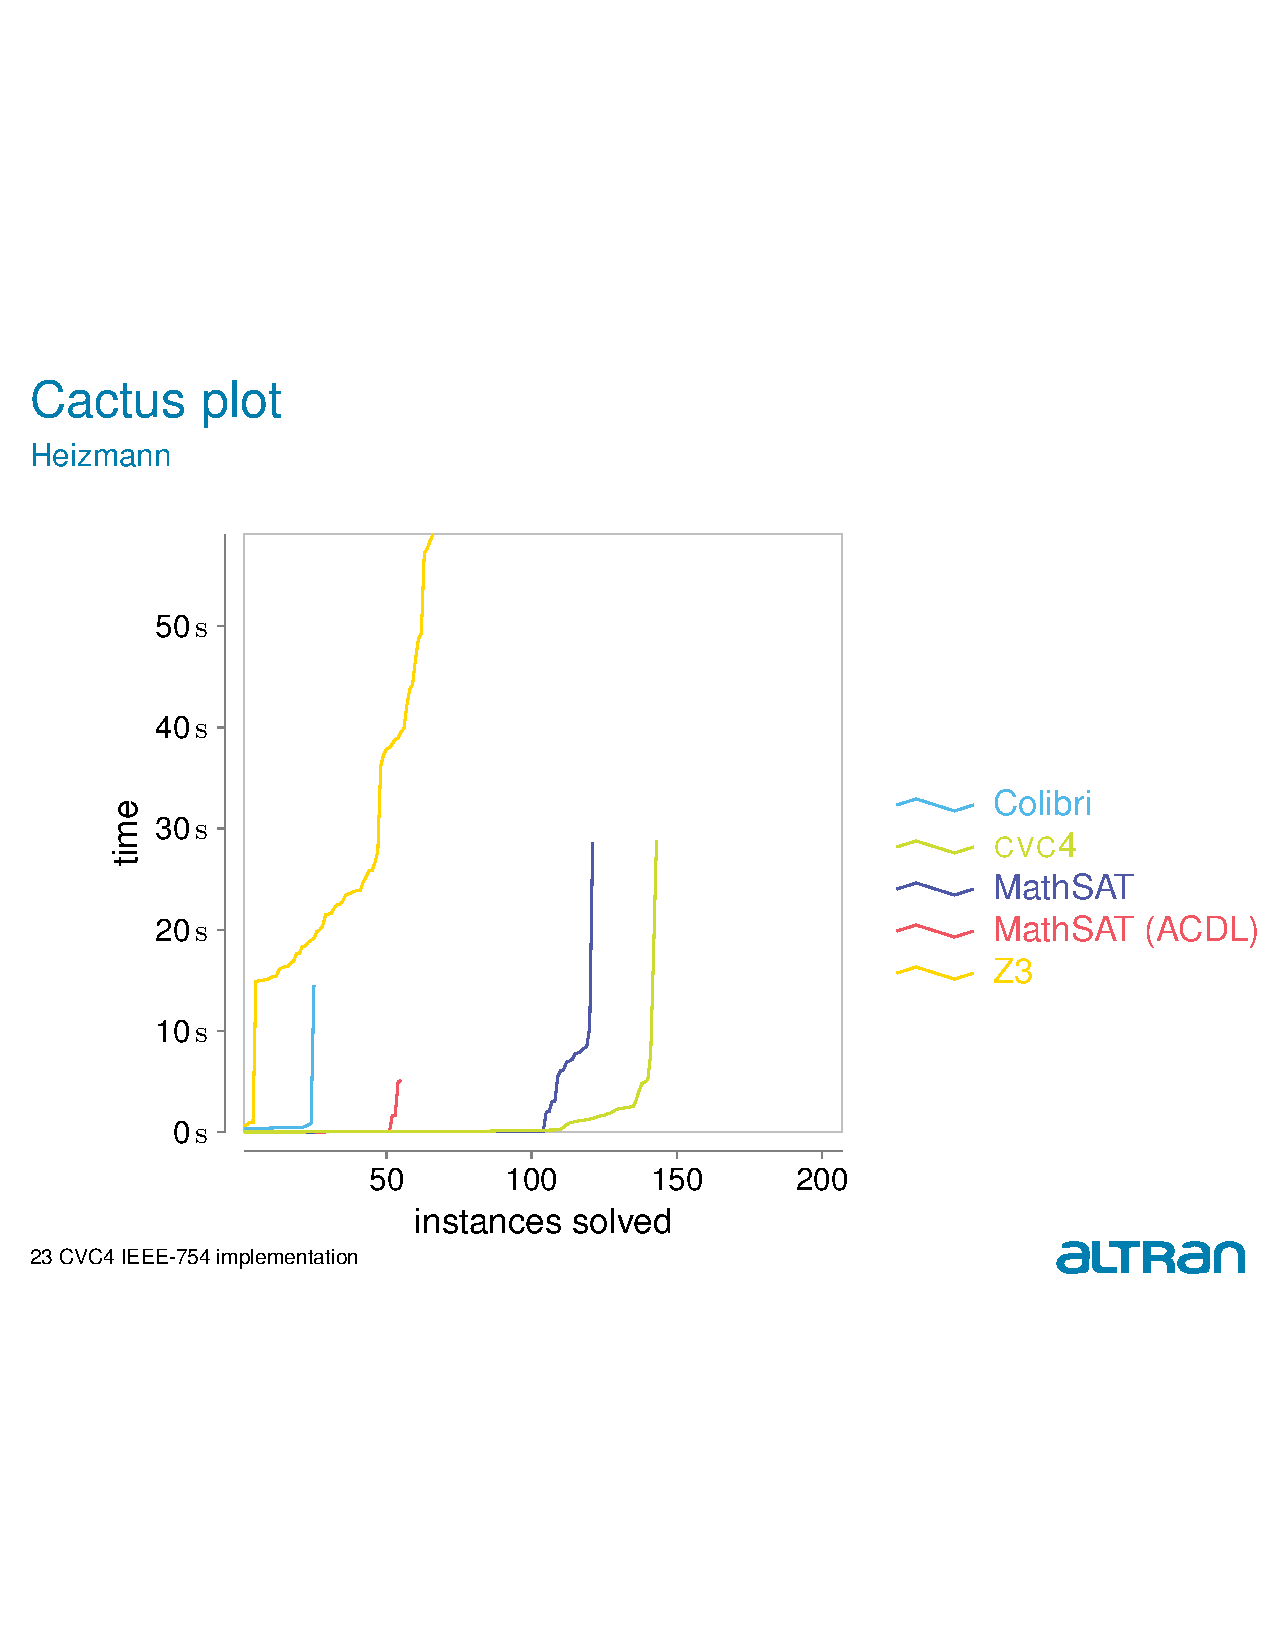
\includegraphics[scale=0.8]{ExtractCVC23.pdf}
\end{figure}\fi
\section{Conclusions}
The SAT community has had substantial experience in measuring, and comparing, solvers whom time is intrinsically variable, and where selective publication of results could be used to justify almost every conclusion: for example selection from the data underpinning Figure \ref{Fig:scatter} could justify anything from ``On UNSAT examples, Solver 1 is comparable to Solver 2'', to ``Solver 2 is thousands of times faster than Solver 1''. If the computer algebra community is to move from publication of a small set of results to more objective comparisons, it will need to develop:
\begin{itemize}
\item significant collections of curated\footnote{The POSSO test suite now seems to exist only in PDF form, at \cite{BiniMourrain1996}.} problem sets, available in a common machine-readable format\footnote{This was one of the original goals of OpenMath \cite{Abbottetal1996}.}, as DIMACS \cite{Spence2015a} and SMT-LIB \cite{Barrettetal2015b} have done for the SAT and SMT communities;
\item the habit of publishing results based on such collections;
\item the habit of publishing more than just averages, and this paper is an attempt to indicate what has been found useful in the SAT/SMT communities.
\end{itemize}
\subsubsection*{Acknowledgements:}

The authors are supported by the European Union's Horizon 2020 research and innovation programme under grant agreement No H2020-FETOPEN-2015-CSA 712689 (\textsf{SC}$^2$). 
\par
{\bf Supporting Data} are available at \url{10.5281/zenodo.896016}.
%\end{enumerate}
\bibliography{../../../jhd}
\end{document}
\begin{figure}
\caption{}
\includegraphics{}
\end{figure}
